% Runtime view subsection, to be included in architecture.tex

\subsection{Runtime view}
This section covers some of the interactions among the system's components. 

Figure \ref{runeclogin} shows the interaction between modules to achieve the e-Customer login function.

Diagrams in Figures \ref{runecticket} and \ref{runecvisit} represent the different steps needed for getting a ticket or booking a visit for an e-Customer. The core of these processes is the retrieval of stores, done through the following steps:
\begin{itemize}[itemsep=-1mm, topsep=-1mm]
  	\item The Access Request module asks for the localization of the user
  	\item The Store Recommender requests stores close to the user based on the parameters defined by the user (as mean of transport, maximum travel time...)
  	\item The Recommender then queries the database to know which of the candidate stores use CLup
  	\item The returned stores are checked for availability to host more tickets based on the queues and time of visits
  	\item The finally filtered list is then returned to the user
\end{itemize}\vspace{.5\baselineskip}
This order has been defined to offer an incremental filter, allowing to access the maps API only once and limit the accesses to the DB to requests only for previously identified store. Furthermore, the request for stores on a geographic base would be limited anyway even for large cities\textsuperscript{\cite{food}}, as opposed to extracting all stores in the database.

\begin{figure}[h]	
	\centering
	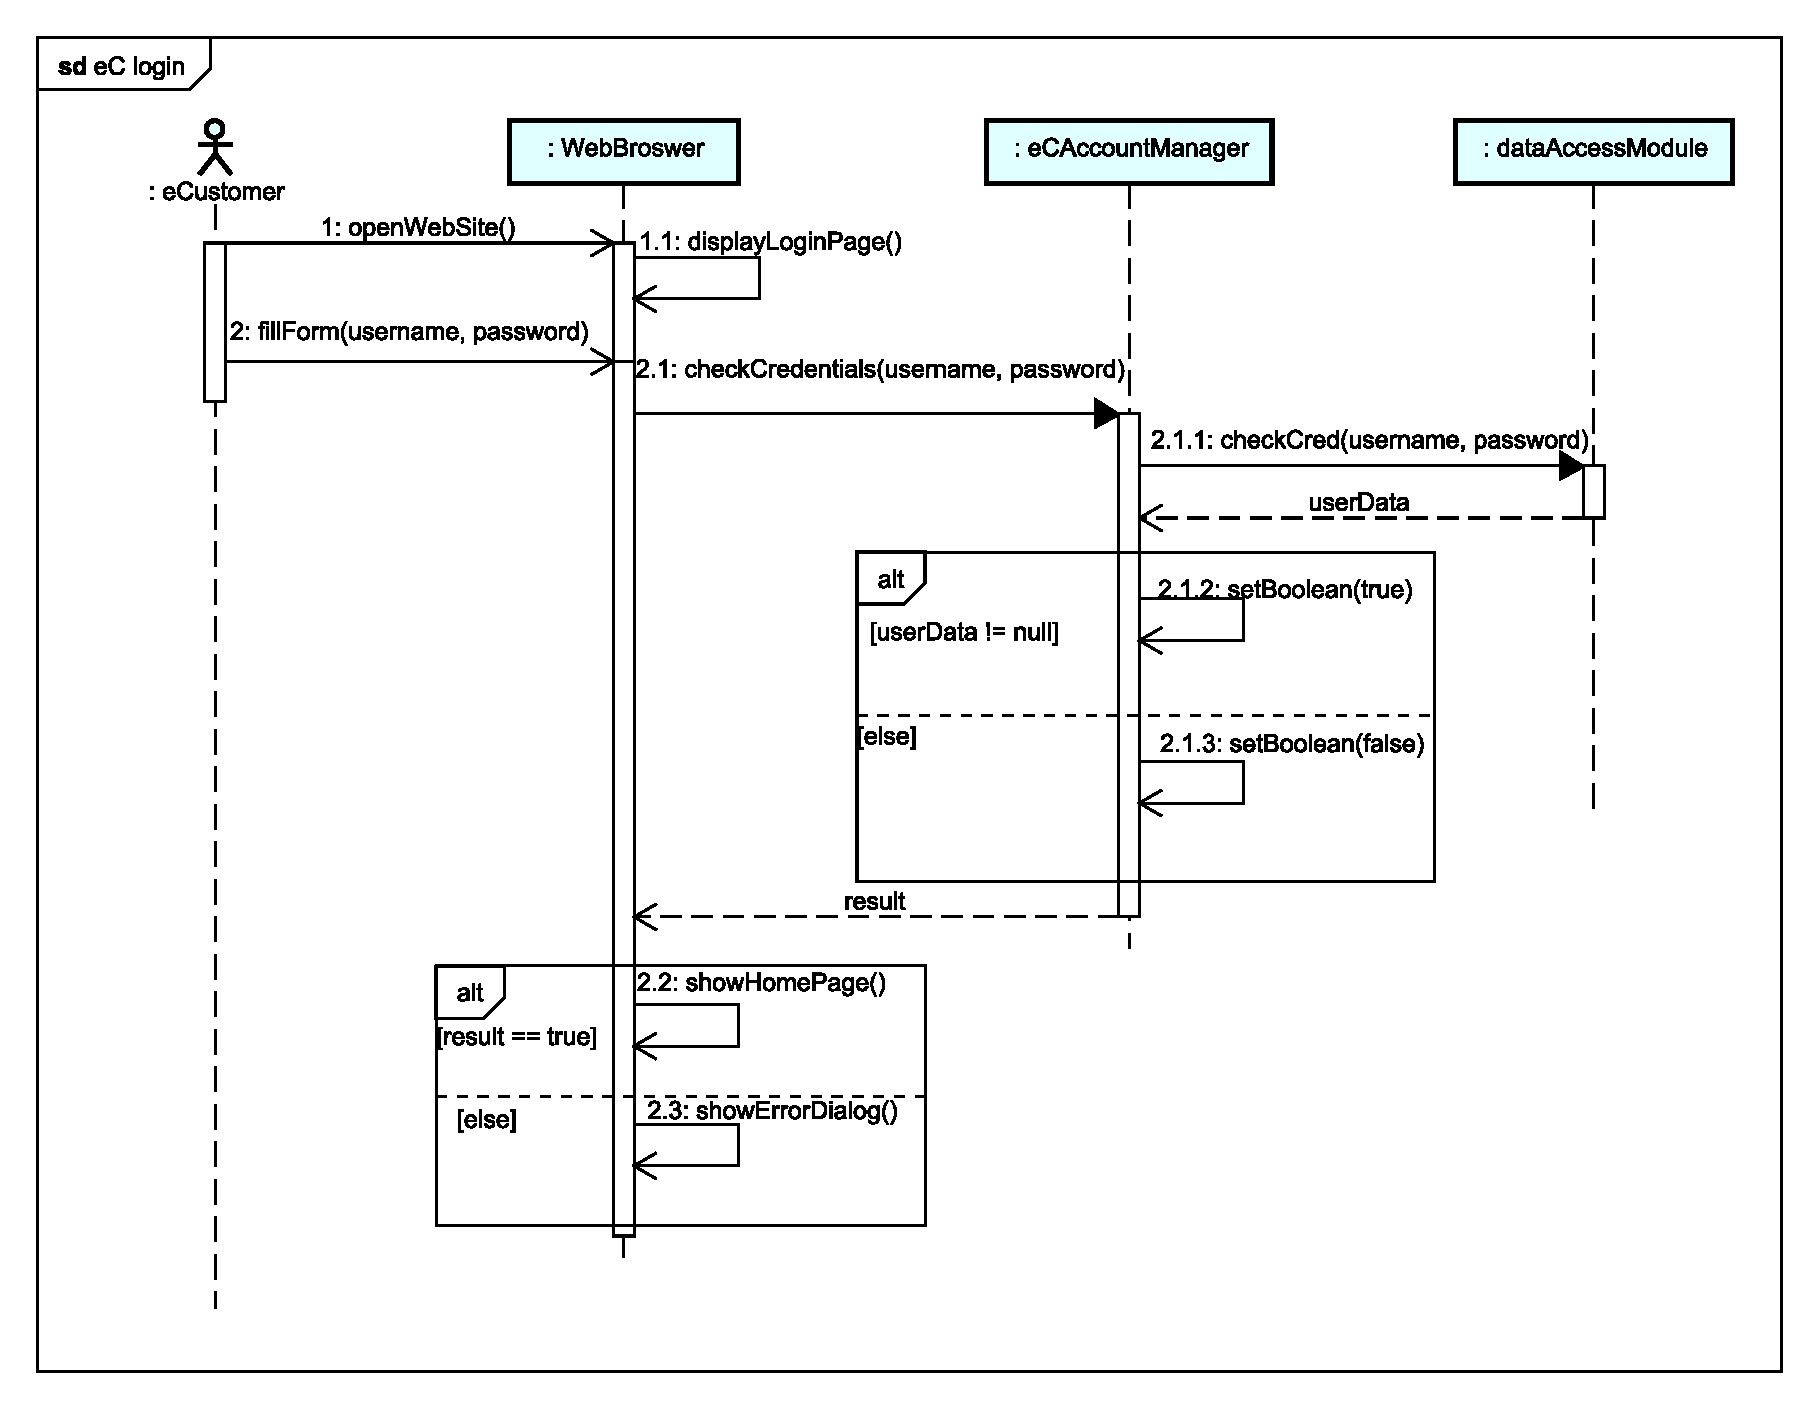
\includegraphics[width=\linewidth] {sequence_diagrams/eC_login_seqD}
	\caption{Runtime view of an e-Customer login}
	\label{runeclogin} 
\end{figure}

\begin{landscape}
	\begin{figure}[p]
		\centering	
		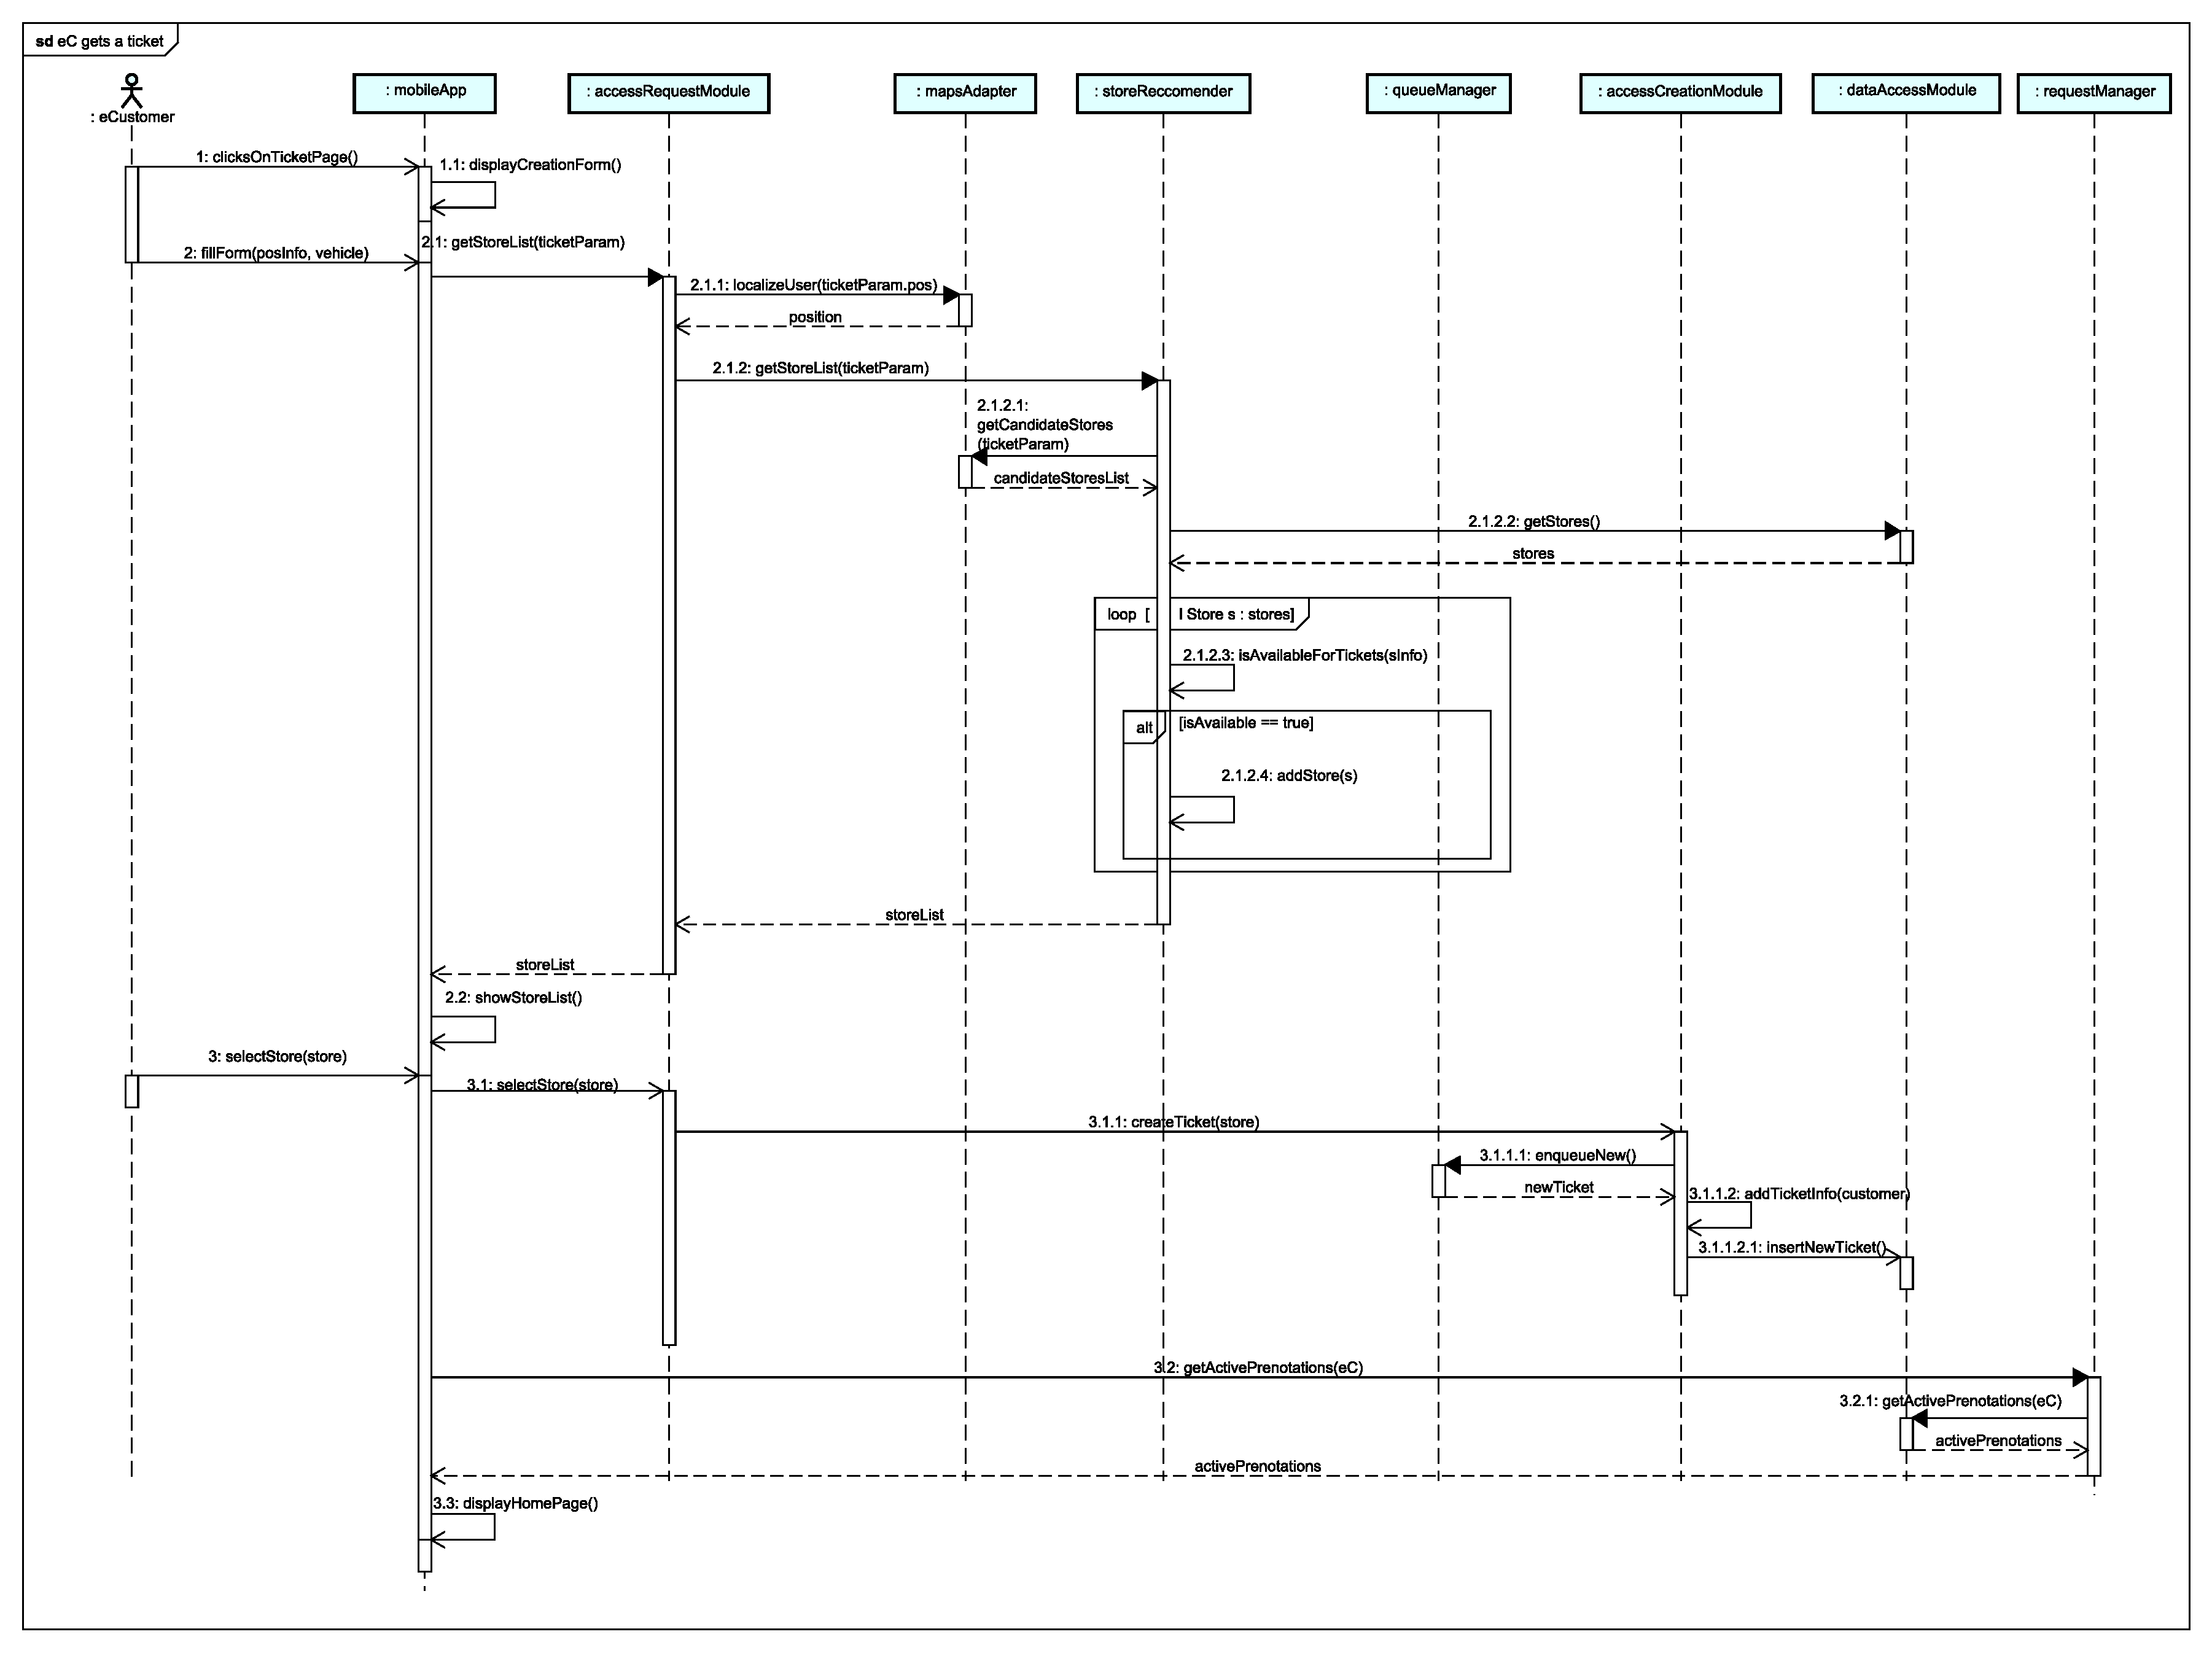
\includegraphics[height=\textheight] {sequence_diagrams/eC_gets_a_ticket_seqD}
		\caption{Runtime view of an e-Customer getting a ticket}
		\label{runecticket} 
	\end{figure}
	
	\begin{figure}[p]
		\centering	
		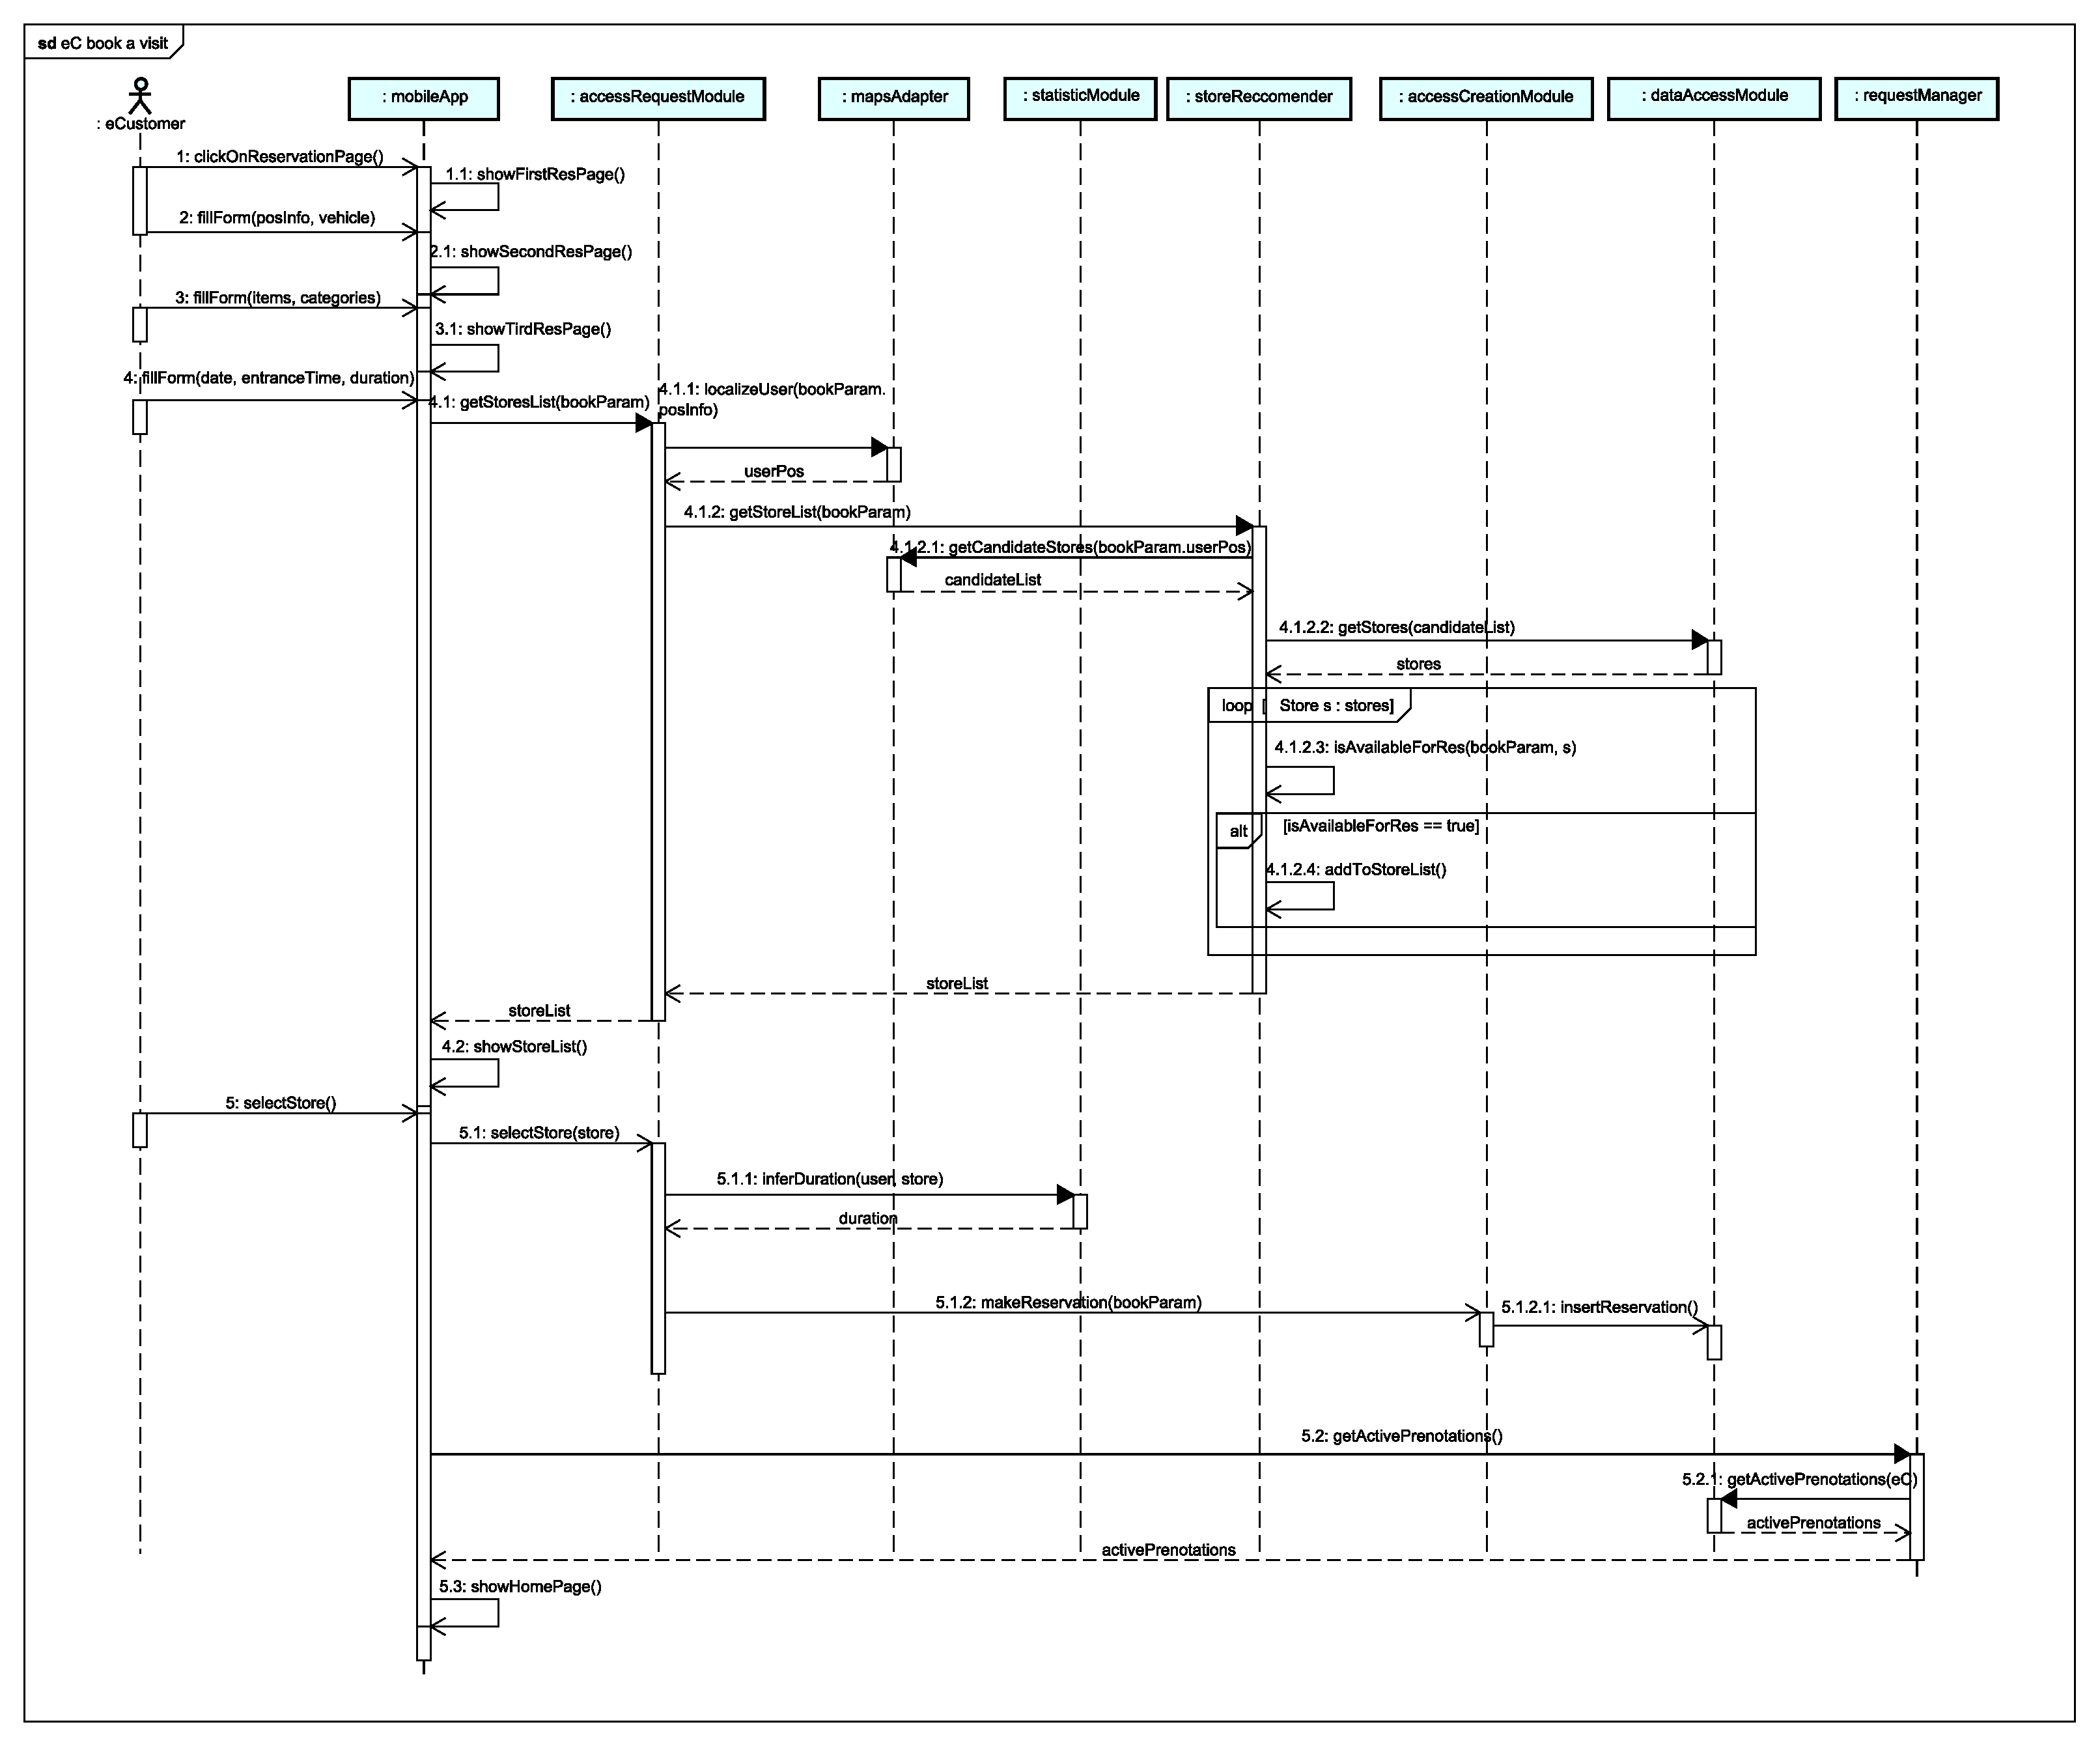
\includegraphics[height=\textheight] {sequence_diagrams/eC_book_a_visit_seqD}
		\caption{Runtime view of an e-Customer booking a visit}
		\label{runecvisit} 
	\end{figure}
\end{landscape}


Figure \ref{ecdelete} illustrates how the request of ticket deletion by an e-Customer is carried out, while Figures \ref{smmodinfo} and \ref{runsmmonitor} concern Store Manager activities, namely modifying their store's information and scanning entering tickets or reservations.

\begin{figure}[h]	
	\centering
	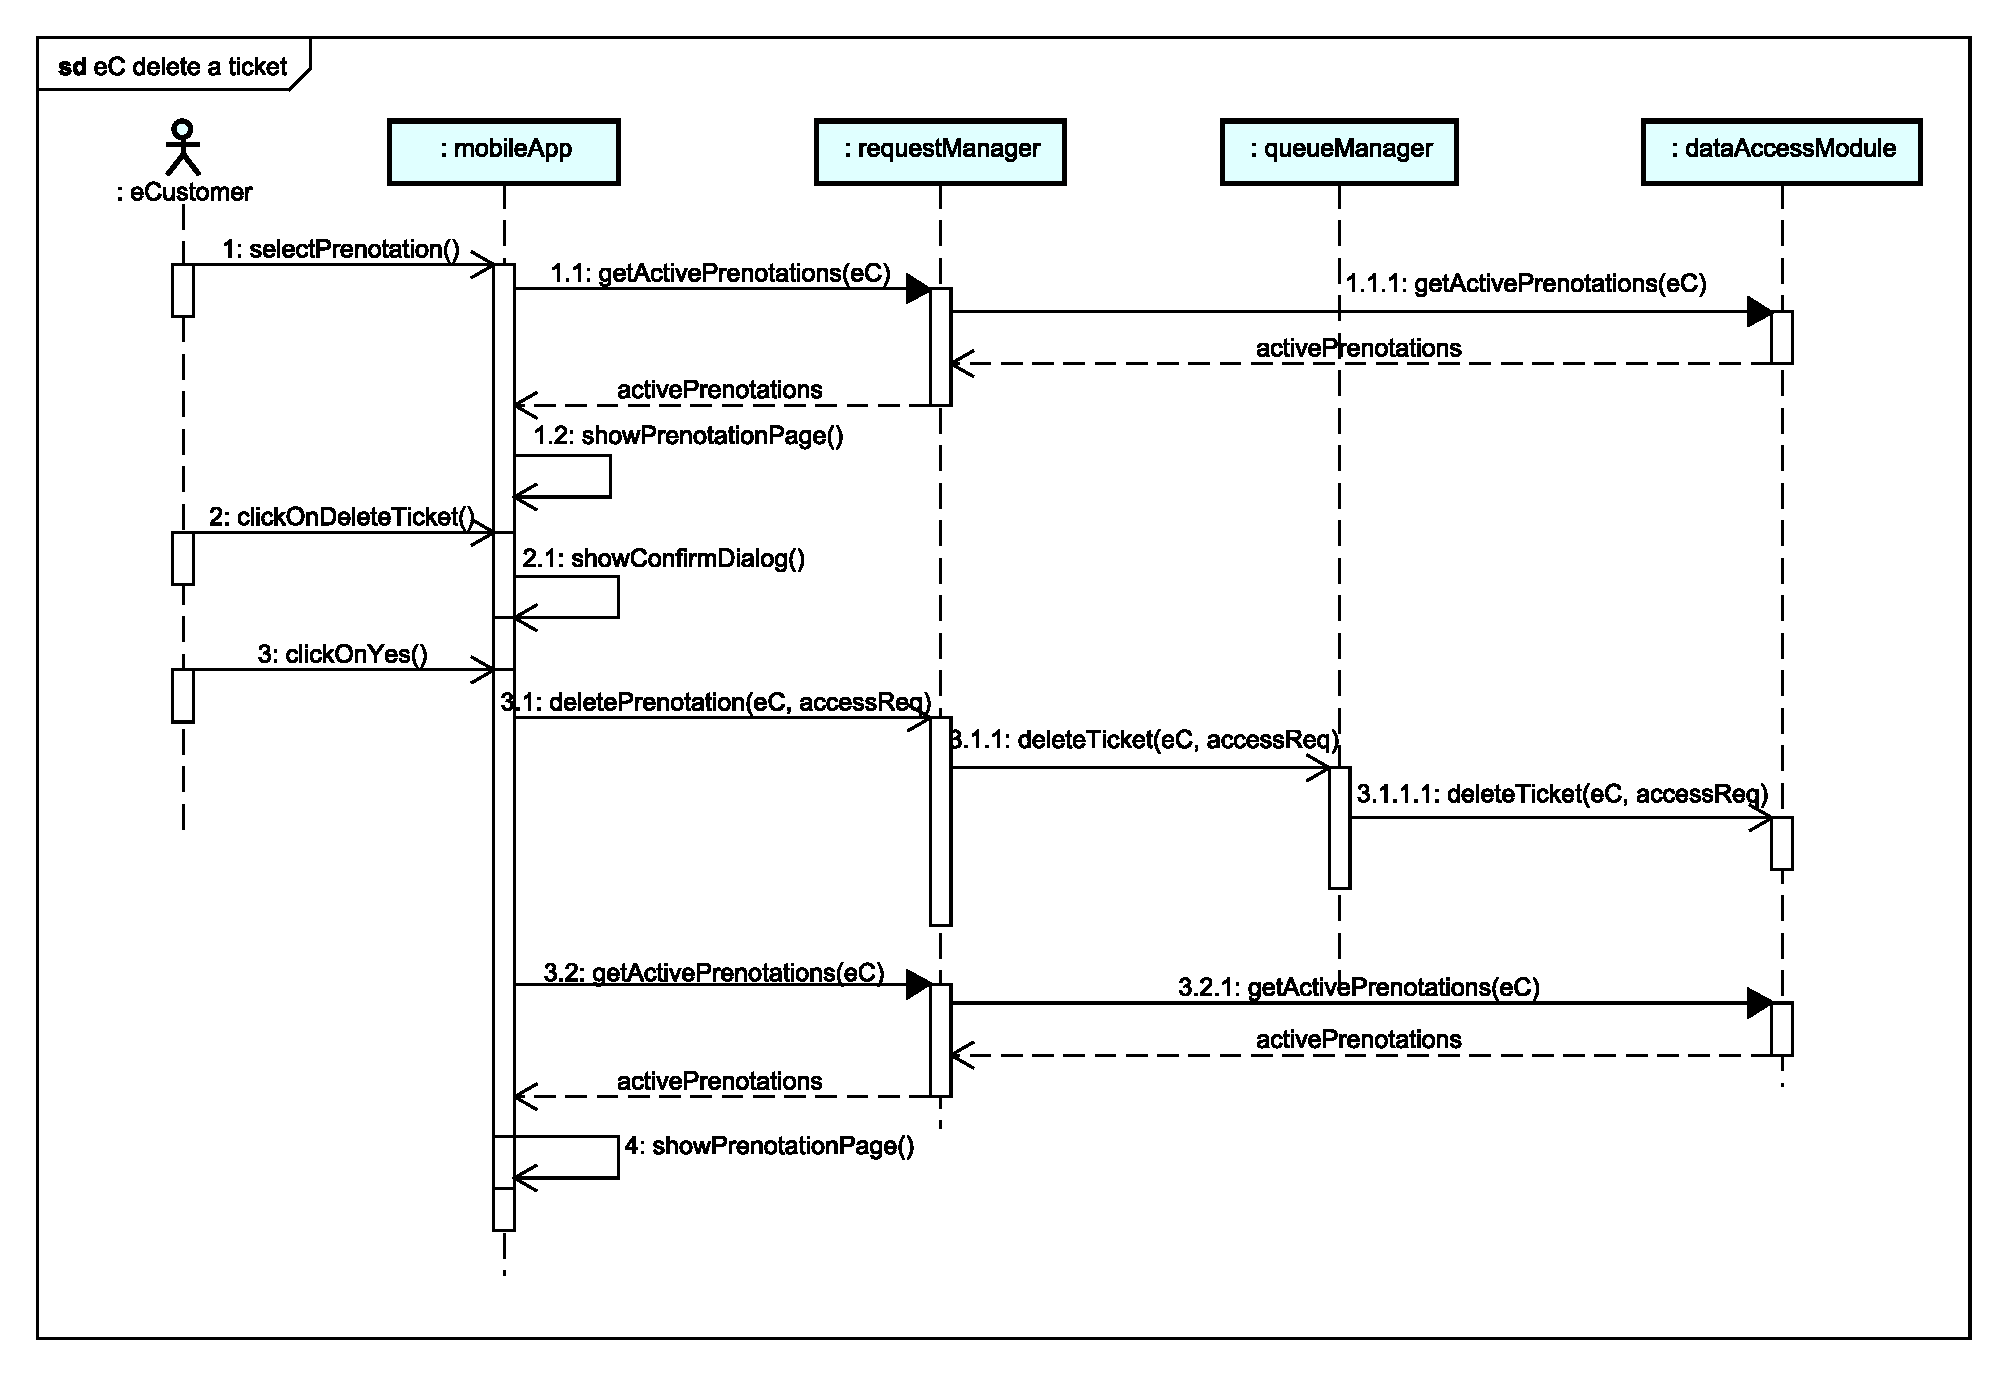
\includegraphics[width=.75\linewidth] {sequence_diagrams/eC_delete_a_ticket_seqD}
	\caption{Runtime view of an e-Customer deleting a ticket}
	\label{ecdelete} 

	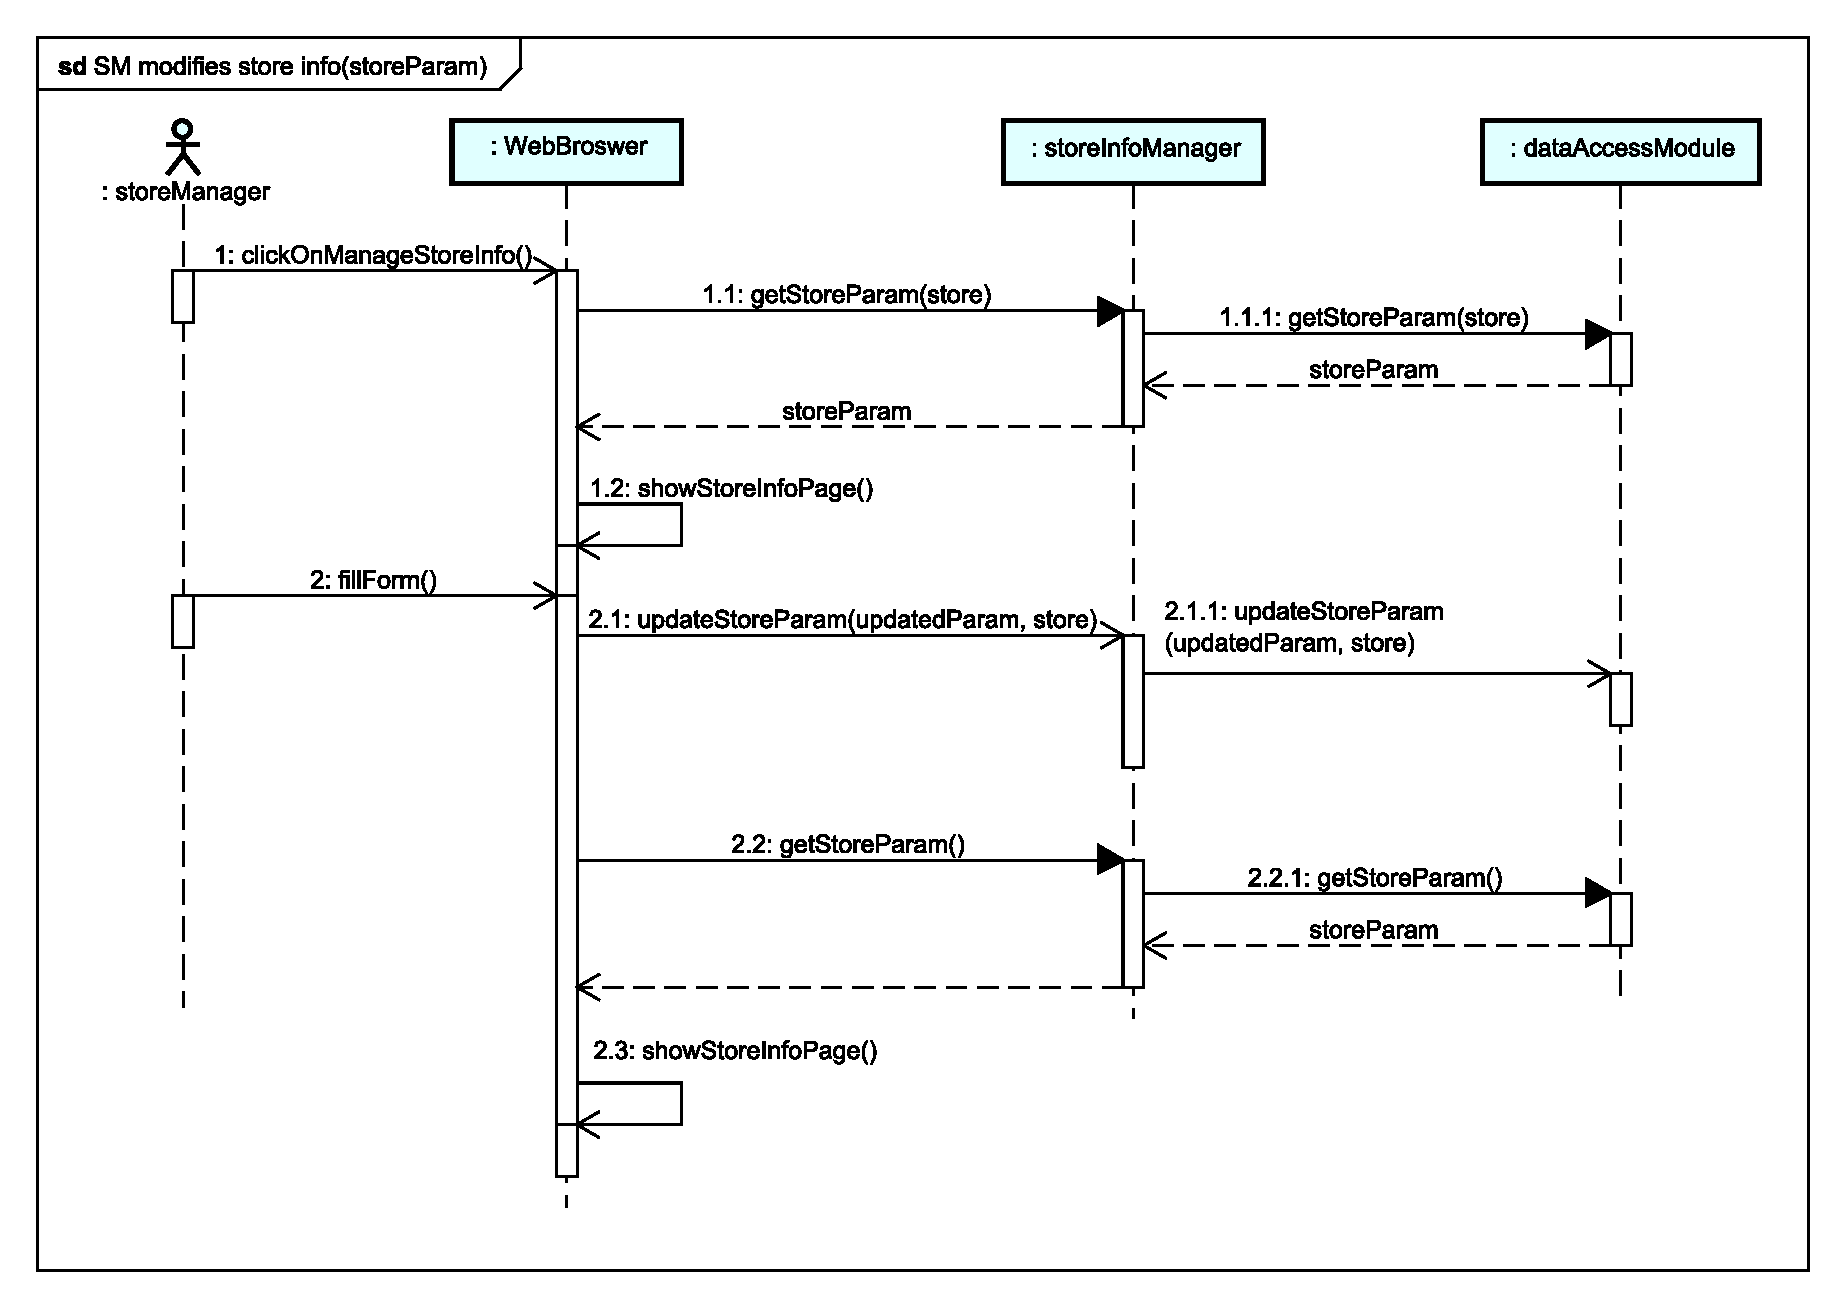
\includegraphics[width=.75\linewidth] {sequence_diagrams/SM_modifies_store_info_seqD}
	\caption{Runtime view of a Store Manager modifying their store's information}
	\label{smmodinfo} 
\end{figure}

\begin{figure}[p]	
	\centering
	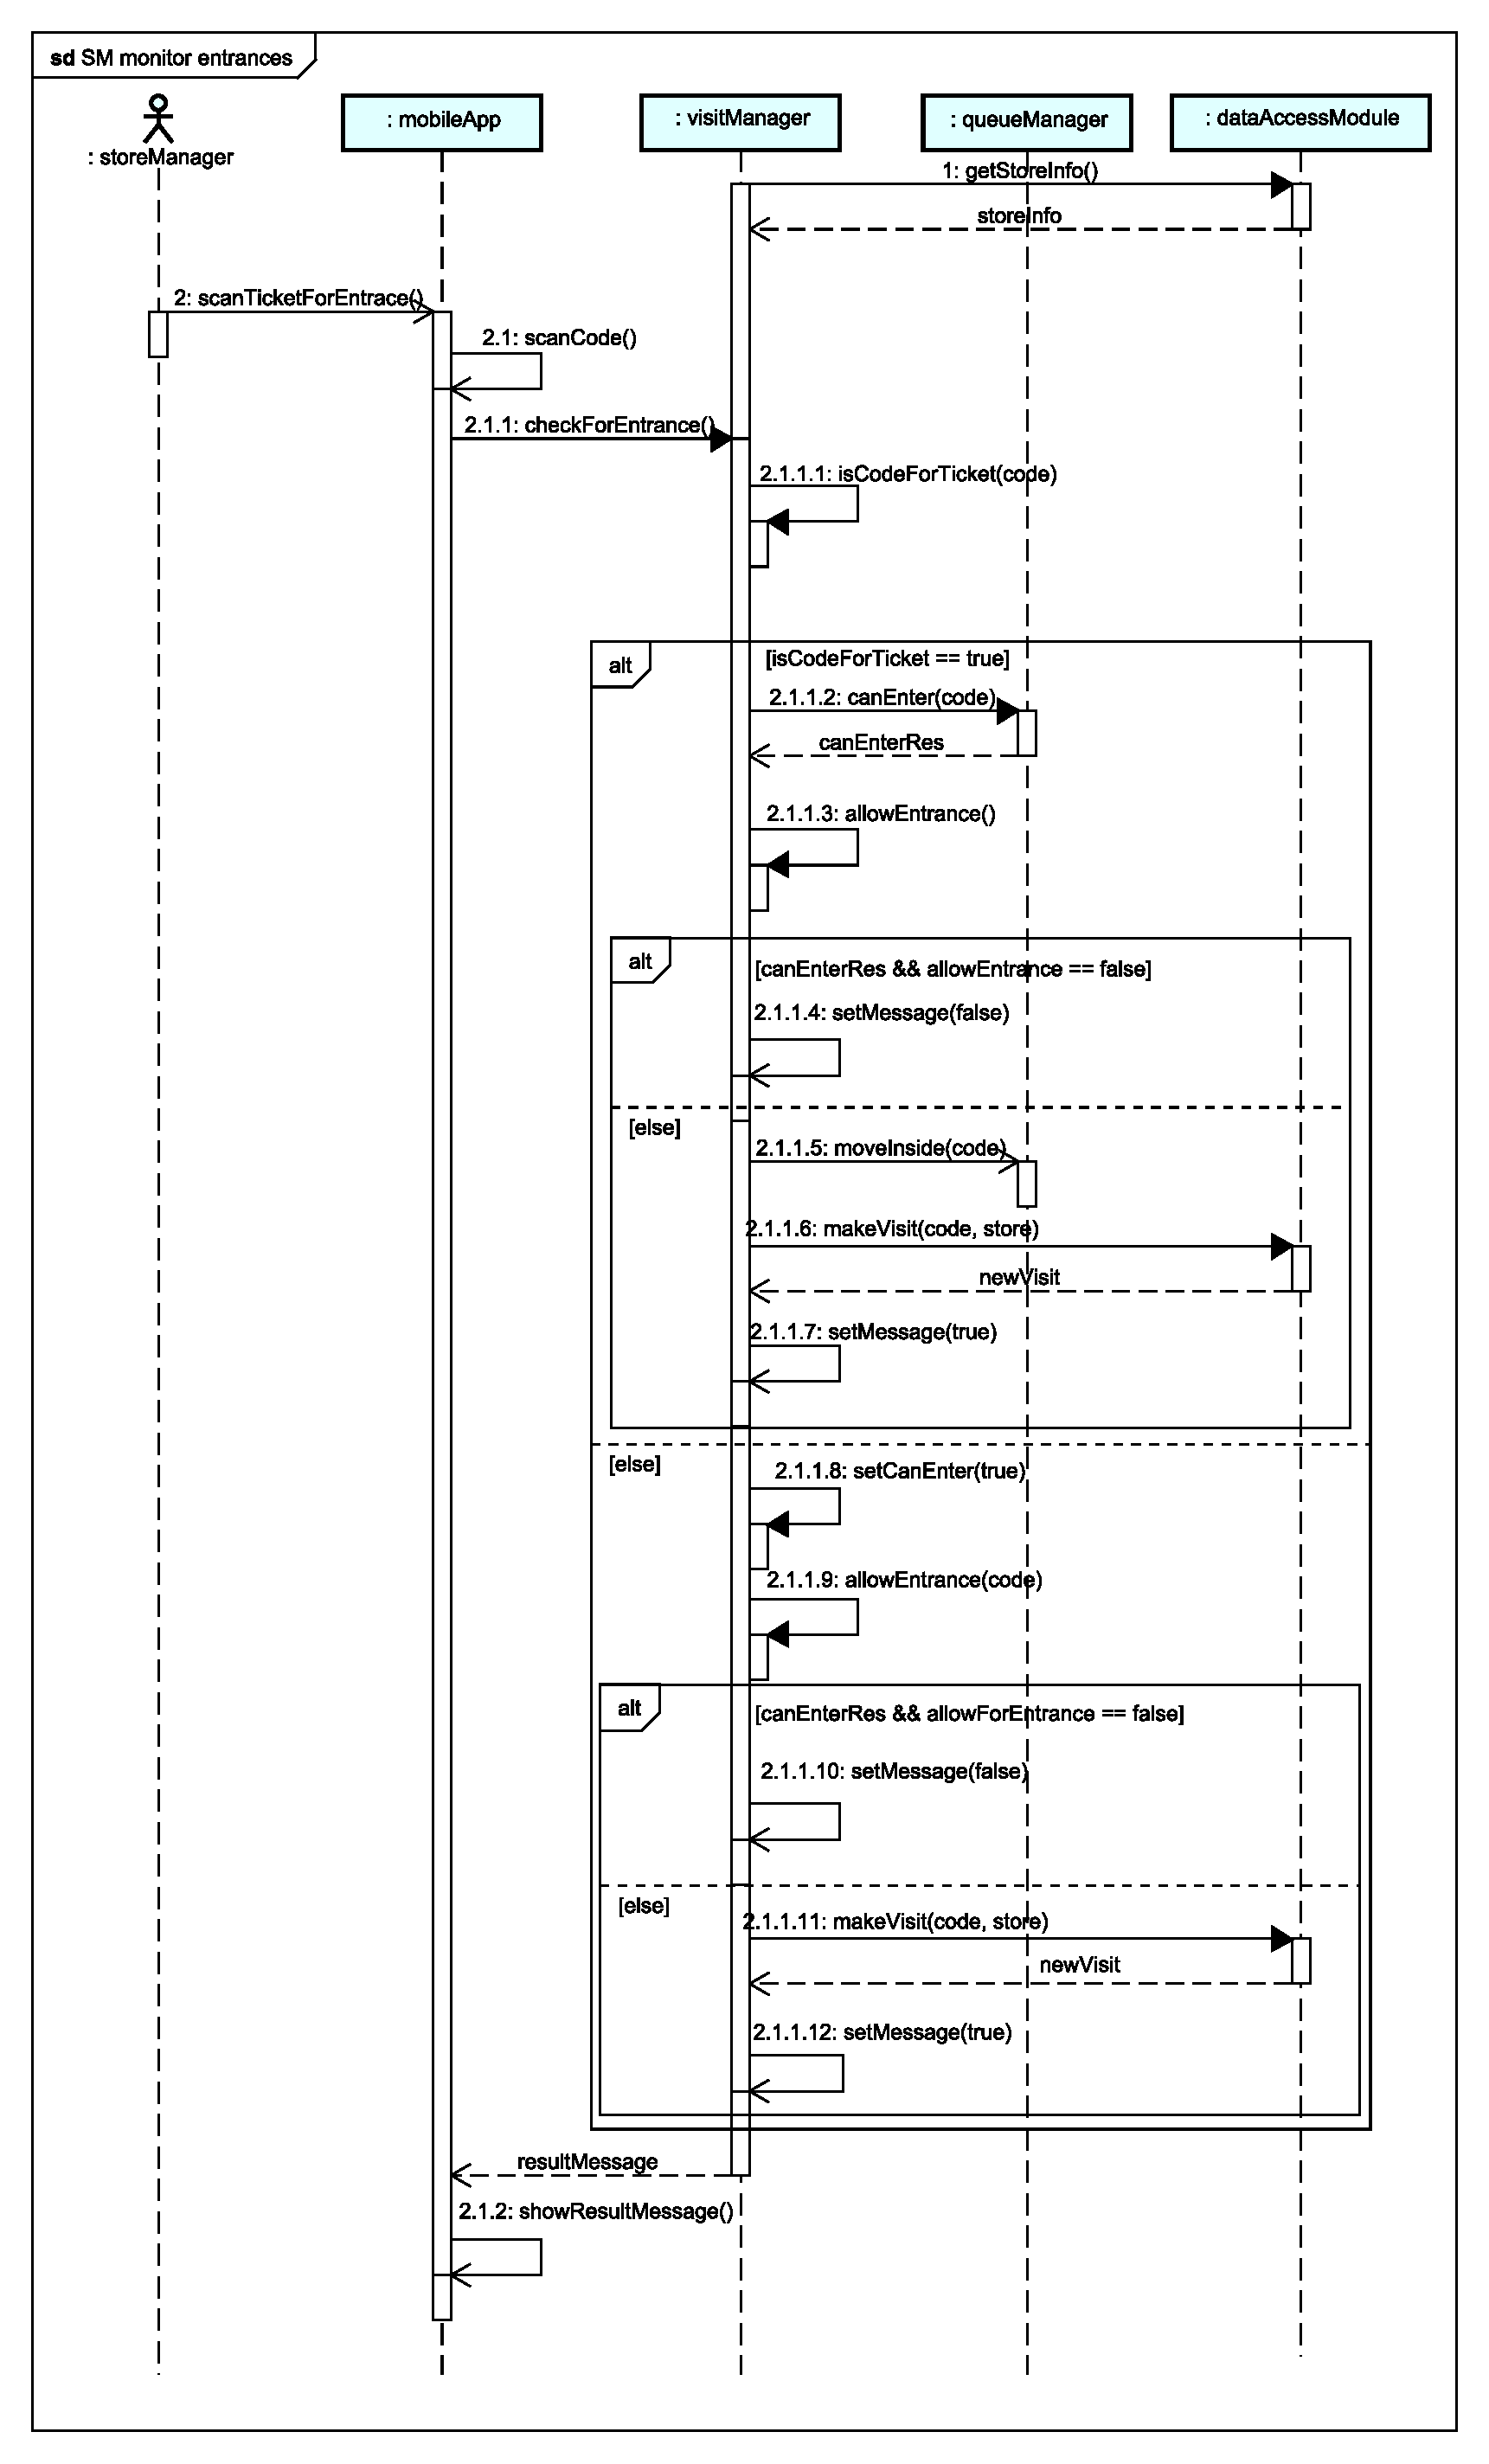
\includegraphics[height=.98\textheight] {sequence_diagrams/SM_monitor_entrances_seqD}
	\caption{Runtime view of a Store Manager monitoring accesses}
	\label{runsmmonitor} 
\end{figure}

\clearpage